\documentclass{article}
\usepackage{xeCJK}
\setmainfont{KaiTi}

\begin{document}
\tableofcontents
\newpage

\section{SLAM Karto}
\subsection{scan matching}
Lu和Milios使用ICP算法计算两个点云之间的位置变换,Karto使用的方法为互相关的方法并被Olson扩展,给出了一定范围之内全局最优解的一种非常有效的方法,并且给出了非常精确的相关系数。
\subsubsection{概率框架}
如图1所示,机器人从$x_{i-1}$运动到$x_i$,运动为$u$,观测值$z$和环境模型$m$以及机器人的位置无关。

整个框架的目标是计算机器人位置的后验分布$p(x_i|x_{i-1},u,m,z)$,利用$Bayes$公式,得到
\begin{equation}
	p(x_i |x_{i-1},u,m,z)\propto p(z|x_i, m)p(x_i|x_{i-1},u)
	\label{eq:bayes_formulation}
\end{equation}

\begin{figure}[h]
	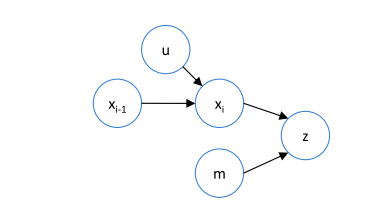
\includegraphics{images/motion_model.png}
	\caption{机器人运动模型示意图}
\end{figure}

公式(\ref{eq:bayes_formulation})中$p(z|x_i,m)$是观测模型:第二项$p(x_i|x_{i-1},u)$是机器人的运动模型。典型的运动模型为多变量高斯分布,而观测模型一般来说更难计算而且在结构上更加的复杂。这篇文章给出了一种高效计算分布$p(z|x_i,m)$的方法。

\subsubsection{查表法栅格化}


\subsection{SPA}


\section{gmapping}
\subsection{}
\end{document}

